\section{Einführung}

\noindent
Vor der Erstellung einer Software muss zunächst ermittelt werden, was der Kunde sich wünscht.\\
Werden die Bedürfnisse des Kunden mit der Softwarelösung nicht befriedigt, gilt das Projekt als gescheitert oder es sind i.d.R. aufwändige (Zeit, Kosten) Nacharbeiten nötig.\\

\vspace{5mm}
\begin{tcolorbox}
    \textbf{Requirements Engineering} ist das systematische Vorgehen des Ermittelns von Anforderungen,
    wobei mit möglichst geringem Aufwand alle notwendigen Informationen gesammelt und schriftlich festgehalten werden.
\end{tcolorbox}
\vspace{5mm}

\noindent
Während sich Fehler im Quellcode zumeist nur auf die \textit{Implementierung} bzw. das \textit{Testing} auswirkt, sind Fehler in den Anforderungen\footnote{
hiermit sind nicht nur logische Fehler gemeint: \textit{Fehler} umfasst in diesem Sinne auch das Fehlen von Informationen
} weitaus teurer: Fallen sie erst in einer späten Phase auf, müssen ggf. relevante Teilsysteme neu durchdacht werden, oder es müssen ganze Phasen neu durchlaufen werden.\\
Fehler in den Anforderungen wirken sich also i.d.R. auf alle Phasen aus, und je später sie erkannt werden, desto aufwändiger wird eine Anpassung (s. Abbildung~\ref{fig:aufwand}).

\begin{figure}
    \centering
    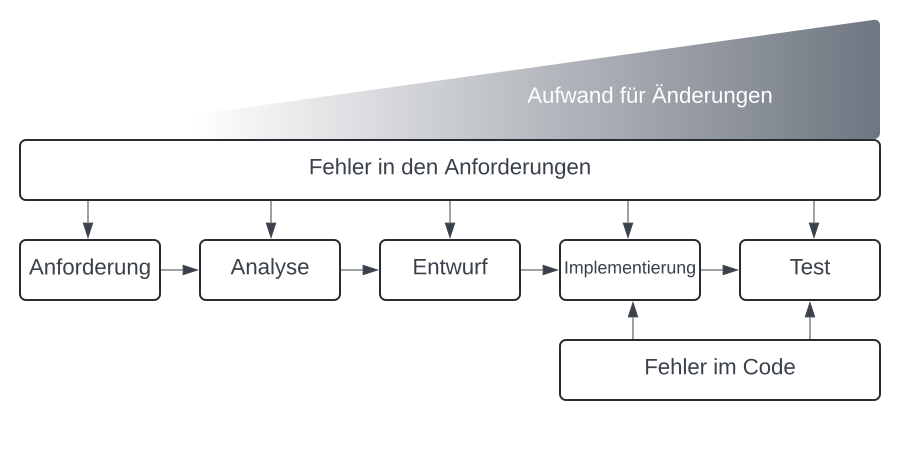
\includegraphics[scale=0.4]{part one/Requirements Engineering/img/aufwand}
    \caption{Je später Änderungen durchgeführt werden müssen, die sich durch fehlerhafte Anforderungen ergeben, desto aufwändiger wird es. (Quelle: in Anlehnung an \cite[38 f., Abb. 4.1 und 4.2]{Wed09})}
    \label{fig:aufwand}
\end{figure}

\noindent
Trotzdem dürfen und müssen Änderungen an den Anforderungen auch noch nach der Anforderungsphase möglich sein.
Deshalb muss das Projekt und das Produkt so organisiert sein, dass diese Änderungen mit möglichst geringem Aufwand möglich sind.\\
Es gilt aber in jedem Fall: Je genauer die Anforderungen zu Beginn des Projektes spezifiziert sind, desto weniger Aufwand benötigt die Umsetzung.\\


\subsubsection*{Kunde muss beraten werden}
Anwender und Kunden sind meistens nicht in der Lage, anhand von abstrakten Modellen und Dokumenten im Voraus alle Eigenschaften und Funktionalitäten einer Software zu definieren.\\
Entwickler und Fachexperten sind deshalb gefragt, zusammen mit Kunde und Anwendern die Anforderungen zu erarbeiten und die \textbf{Machbarkeit} zu überprüfen.\\


\subsubsection*{Verantwortlichkeit des Kunden}
Kunden müssen sich gleichzeitig in der Pflicht sehen, den Entwicklern während der Anforderungsanalyse sein Geschäftsfeld zu erklären\footnote{
die Fachlichkeit sollte sich der Entwickler selber aneignen; in weiteren Phasen können Details mit Fachexperten besprochen werden, im günstigsten Fall noch im Entwurf
}.\\
Auch die Mitarbeiter des Kunden müssen sich aktiv beteiligen um klären zu können, was zuerst gemacht werden soll, bzw. wie in den ersten Schritten priorisiert werden soll.
Rechtzeitige Entscheidungen helfen dabei, zielgerichtet umzusetzen.\\


\subsubsection*{Arbeiten ohne Anforderungen geht nicht}
Werden keine Absprachen getroffen kann es sein, dass der Entwickler nur eine sehr begrenzte Idee dessen hat, was umzusetzen ist, bzw. wie die abzubildenden Prozesse ineinandergreifen.\\
Das kann dazu führen, dass das fertige Produkt unbrauchbar ist oder zuviel Aufwand in Änderungen investiert werden muss, womit die Wirtschaftlichkeit des Projektes gefährdet ist.\\

\noindent
Zur Lösung solcher Probleme bietet es sich an

\begin{itemize}
    \item Aufwand für Anforderungen so gering wie möglich aber so umfangreich wie nötig halten - braucht der Kunde bspw. eine umfangreiche, normierte, bis in das kleinste Detail spezifizierte Dokumentation?
    \item Tabellarisch und mit durchdachten Vorlagen arbeiten
    \item Auftrag nicht annehmen, da spätere Leistungen durch Anpassungen nicht bezahlt werden, oder Streitigkeiten über die Vertragsbedingungen auftreten können
\end{itemize}


\subsubsection*{Schriftliche Dokumentation hilft}
Eine Dokumentation der Anforderung in Schriftform kann eine Hilfe für die Kommunikation mit dem Kunden sein.\\
Außerdem hilft sie, Mißverständnisse zu vermeiden und kann als Referenz für (zukünftige) Entwickler dienen, z.b. bei Rückfragen, oder wenn es um die Wartung der Software geht (\textit{wie} soll \textit{was} funktionieren).\\


\subsubsection*{Wer ist der Kunde?}
Anforderungen des \textbf{Kunden} können sich von den Anforderungen des \textbf{Endanwenders} unterscheiden.
In \cite[41]{Wed09} ist das Beispiel von einem Spiele-Publisher und dem Anwender gegeben, bei dem der Publisher möglichst viel Geld mit den Spielen verdienen will, der Anwender aber in erster Linie möglichst viel Spaß mit dem Spiel haben möchte.
